\documentclass{beamer}
%\usetheme{Boadilla}
\usepackage[latin1]{inputenc}
\usepackage{ upgreek }
\usepackage{verbatim} 
\usepackage{amsmath}

\usepackage{amssymb}
\usepackage{graphicx}
\usepackage{url}
\usepackage{verbatim} 

\DeclareMathOperator*{\argmax}{argmax}
\DeclareMathOperator*{\argmin}{argmin}  

\usetheme{Warsaw}
\title{Semantic Labeling of 3D Point Clouds for Indoor Scenes}



\newcommand{\n}{{n}}             % number of training examples
\newcommand{\x}{{\mathbf x}}     % segmented scene
\newcommand{\xs}[1]{{x_{#1}}}    % segment of scene
\newcommand{\y}{{\mathbf y}}     % labeling of scene
\newcommand{\ys}[1]{{y_{#1}}}    % labeling of segment
\newcommand{\ysc}[2]{{y_{#1}^{#2}}}    % indicator of class label of segment
\newcommand{\zsc}[2]{{z_{#1}^{#2}}}    % indicator of class label pair
\newcommand{\fn}[1]{{\phi_n(#1)}}      % feature function for segment node
\newcommand{\fe}[3]{{\phi_{#1}(#2,#3)}}% feature function for edge
\newcommand{\w}{{\mathbf w}}           % full weight vector
\newcommand{\wn}[1]{{w_n^{#1}}}        % weight vector of segment node
\newcommand{\we}[3]{{w_{#1}^{#2#3}}}   % weight vector of edge
\newcommand{\df}[3]{{f_{#3}(#1,#2)}}   % discriminant function
\newcommand{\loss}[2]{{\Delta(#1,#2)}}   % discriminant function



\begin{document}
\begin{frame}
\titlepage
\end{frame}

\begin{frame}{Motivation}
	\begin{figure}[t!]
		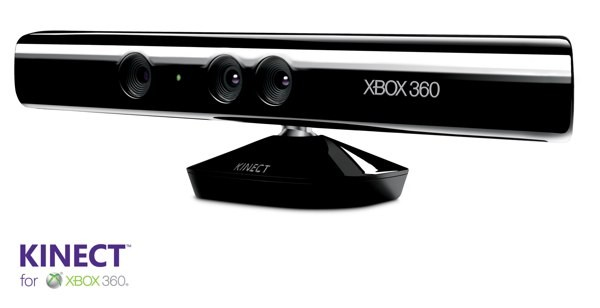
\includegraphics[width=.5\linewidth]{kinect.jpg}
	\end{figure}

	\begin{itemize}
		\item 3D era for robots has arrived 
		\item  cheap, fast 3D machine vision
		\item  both color and depth available
	\end{itemize}

\end{frame}

\begin{frame}{Introduction}
	\begin{itemize}
		\item How does a kinect pointcloud look like? \footnote{http://arstechnica.com/gaming/news/2010/11/bathed-in-light-how-the-kinect-paints-your-room-in-ir-video.ars}

	\end{itemize}
\end{frame}

\begin{frame}{Introduction}
	\begin{itemize}
		\item Desired goal: labeled pointcloud:(show)

	\end{itemize}
\end{frame}

\begin{frame}{Approach}
	\begin{itemize}
		\item stitching:(show)
		\item  segmentation:(show)
		\item  graph construction(show using graphviz?)
		\item  feature generation
		\item  inference
	\end{itemize}

\end{frame}

\begin{frame}{Captured Properties}
	\begin{itemize}
		\item Visual Appearance
		\item  Local Shape and Geometry
		\item  Geometrical Context
	\end{itemize}

\end{frame}

\begin{frame}{Visual Appearance}
match the following to table/printer
\begin{figure}[t!]

\includegraphics[width=.3\linewidth]{printer-small.png}
\hskip .2in

\includegraphics[width=.3\linewidth]{table-small.png}
\end{figure}
\end{frame}

\begin{frame}{Visual Appearance}

\begin{figure}[t!]
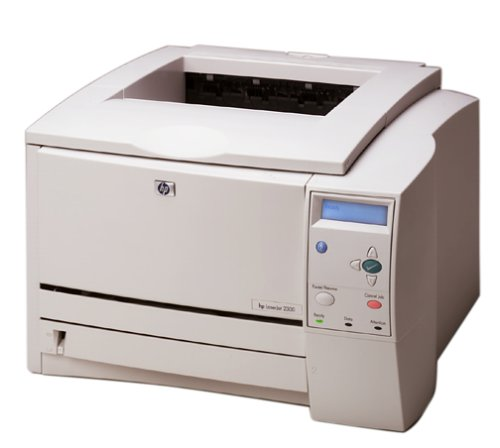
\includegraphics[width=.4\linewidth]{printer.jpg}
\hskip .2in
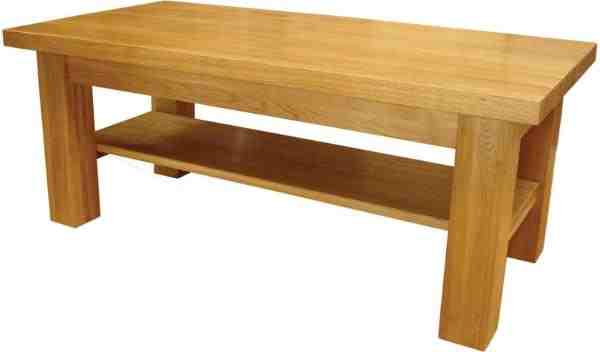
\includegraphics[width=.4\linewidth]{table.jpg}
\end{figure}
\end{frame}

\begin{frame}{Model}
\begin{itemize}

 \item The 3D scene is encoded using Markov Random Field with log-linear node and pairwise edge potentials
 
 % a small graph with objects in the scene representing nodes and edges?
 
\item Goal: Given a segmented point cloud $\x=(\xs{1},...,\xs{N})$  predict a labeling $\y=(\ys{1},...,\ys{N})$

\item where $\ys{i}=(\ysc{i}{1},...,\ysc{i}{K})$,  $ \forall \ysc{i}{k} \in \{0,1\}$ 


\item For a segmented point cloud $\x$, the prediction $\hat{\y}$ is 
\begin{equation} \label{eq:argmax}
\hat{\y} = \argmax_\y \df{\x}{\y}{\w}
\end{equation}

\end{itemize}
\end{frame}


\begin{frame}{Model}
\begin{itemize}

\item Given $(\mathcal{V},\mathcal{E})$, individual segment features $\fn{i}$ and edge features $\fe{t}{i}{j}$

\begin{equation} \label{eq:model}
\begin{split}
\df{\y}{\x}{\w} & = \sum_{i \in \mathcal{V}} \sum_{k=1}^{K} \ysc{i}{k} \left[\wn{k} \cdot \fn{i} \right] \\
 & + \sum_{(i,j)\in \mathcal{E}}   \sum_{T_t \in {\cal T}}  \sum_{(l,k)\in T_t} \ysc{i}{l} \ysc{j}{k}  \left[\we{t}{l}{k} \cdot \fe{t}{i}{j}\right] 
 \end{split}
\end{equation}

\end{itemize}
\end{frame}

\begin{frame}{Model}

\begin{itemize}
%There may be multiple types $t$ of edge feature maps $\fe{t}{i}{j}$, and each type has a graph over the $K$ classes with edges $T_t$. If $T_t$ contains an edge between classes $l$ and $k$, then this feature map and a weight vector $\we{t}{l}{k}$ is used to model the dependencies between classes $l$ and $k$. If the edge is not present in $T_t$, then $\fe{t}{i}{j}$ is not used.

\item Multiple types of edge feature maps $\fe{t}{i}{j}$
\item Each type has a graph over the $K$ classes with edges  $T_t$
\item If $T_t$ contains edge $(l,k)$, then $\fe{t}{i}{j}$ and $\we{t}{l}{k}$  model the dependencies between classes $l$ and $k$.
\item Associative edges:  ${T_t}=\{(k,k)| \forall k=1..K\}$
\item Non-associative edges: $T_t=\{(l,k)| \forall l,k=1..K\}$
\item Object-associate edges: $T_t=\{(l,k) | \exists object , ~ l,k\in {\rm parts}({\rm object})\}$

\end{itemize}
\end{frame}

\begin{frame}{Model}
\begin{itemize}
\item Parsimonious model

\item Two types of feature maps: 
\begin{itemize}
\item ``object-associative'' features $\fe{oa}{i}{j}$ - used between classes that are parts of the same object (e.g., ``chair base'', ``chair back'' and ``chair back rest''). 
\item ``non-associative'' features $\fe{na}{i}{j}$ -  used between any pair of classes.
\end{itemize}
\item Since $|T_{na}| >> |T_{oa}|$ , the number of parameters to learn is lesser compared to modeling all edges as non-associative.
\end{itemize}
\end{frame}


\begin{frame}{Features}

\end{frame}

\begin{frame}{Learning}

\end{frame}

\begin{frame}{Inference}
 
 
\end{frame}

\begin{frame}{Data}
% types and number of scene 
% examples of labeled pointclouds

\end{frame}


\begin{frame}{Results }
% put table
% put confusion matrices 
% discuss the points mentioned in the paper  
\end{frame}

\begin{frame}{Robotic Experiments}
% setup
%demo
% table of results
\end{frame}

\begin{frame}{Current Work: }
\end{frame}

\begin{frame}{Current Work: }
\end{frame}

\end{document} 
